\documentclass[twoside]{book}

% Packages required by doxygen
\usepackage{fixltx2e}
\usepackage{calc}
\usepackage{doxygen}
\usepackage[export]{adjustbox} % also loads graphicx
\usepackage{graphicx}
\usepackage[utf8]{inputenc}
\usepackage{makeidx}
\usepackage{multicol}
\usepackage{multirow}
\PassOptionsToPackage{warn}{textcomp}
\usepackage{textcomp}
\usepackage[nointegrals]{wasysym}
\usepackage[table]{xcolor}

% Font selection
\usepackage[T1]{fontenc}
\usepackage[scaled=.90]{helvet}
\usepackage{courier}
\usepackage{amssymb}
\usepackage{sectsty}
\renewcommand{\familydefault}{\sfdefault}
\allsectionsfont{%
  \fontseries{bc}\selectfont%
  \color{darkgray}%
}
\renewcommand{\DoxyLabelFont}{%
  \fontseries{bc}\selectfont%
  \color{darkgray}%
}
\newcommand{\+}{\discretionary{\mbox{\scriptsize$\hookleftarrow$}}{}{}}

% Page & text layout
\usepackage{geometry}
\geometry{%
  a4paper,%
  top=2.5cm,%
  bottom=2.5cm,%
  left=2.5cm,%
  right=2.5cm%
}
\tolerance=750
\hfuzz=15pt
\hbadness=750
\setlength{\emergencystretch}{15pt}
\setlength{\parindent}{0cm}
\setlength{\parskip}{3ex plus 2ex minus 2ex}
\makeatletter
\renewcommand{\paragraph}{%
  \@startsection{paragraph}{4}{0ex}{-1.0ex}{1.0ex}{%
    \normalfont\normalsize\bfseries\SS@parafont%
  }%
}
\renewcommand{\subparagraph}{%
  \@startsection{subparagraph}{5}{0ex}{-1.0ex}{1.0ex}{%
    \normalfont\normalsize\bfseries\SS@subparafont%
  }%
}
\makeatother

% Headers & footers
\usepackage{fancyhdr}
\pagestyle{fancyplain}
\fancyhead[LE]{\fancyplain{}{\bfseries\thepage}}
\fancyhead[CE]{\fancyplain{}{}}
\fancyhead[RE]{\fancyplain{}{\bfseries\leftmark}}
\fancyhead[LO]{\fancyplain{}{\bfseries\rightmark}}
\fancyhead[CO]{\fancyplain{}{}}
\fancyhead[RO]{\fancyplain{}{\bfseries\thepage}}
\fancyfoot[LE]{\fancyplain{}{}}
\fancyfoot[CE]{\fancyplain{}{}}
\fancyfoot[RE]{\fancyplain{}{\bfseries\scriptsize Generated by Doxygen }}
\fancyfoot[LO]{\fancyplain{}{\bfseries\scriptsize Generated by Doxygen }}
\fancyfoot[CO]{\fancyplain{}{}}
\fancyfoot[RO]{\fancyplain{}{}}
\renewcommand{\footrulewidth}{0.4pt}
\renewcommand{\chaptermark}[1]{%
  \markboth{#1}{}%
}
\renewcommand{\sectionmark}[1]{%
  \markright{\thesection\ #1}%
}

% Indices & bibliography
\usepackage{natbib}
\usepackage[titles]{tocloft}
\setcounter{tocdepth}{3}
\setcounter{secnumdepth}{5}
\makeindex

% Hyperlinks (required, but should be loaded last)
\usepackage{ifpdf}
\ifpdf
  \usepackage[pdftex,pagebackref=true]{hyperref}
\else
  \usepackage[ps2pdf,pagebackref=true]{hyperref}
\fi
\hypersetup{%
  colorlinks=true,%
  linkcolor=blue,%
  citecolor=blue,%
  unicode%
}

% Custom commands
\newcommand{\clearemptydoublepage}{%
  \newpage{\pagestyle{empty}\cleardoublepage}%
}

\usepackage{caption}
\captionsetup{labelsep=space,justification=centering,font={bf},singlelinecheck=off,skip=4pt,position=top}

%===== C O N T E N T S =====

\begin{document}

% Titlepage & ToC
\hypersetup{pageanchor=false,
             bookmarksnumbered=true,
             pdfencoding=unicode
            }
\pagenumbering{roman}
\begin{titlepage}
\vspace*{7cm}
\begin{center}%
{\Large pinocchio\+\_\+bullet }\\
\vspace*{1cm}
{\large Generated by Doxygen 1.8.11}\\
\end{center}
\end{titlepage}
\clearemptydoublepage
\tableofcontents
\clearemptydoublepage
\pagenumbering{arabic}
\hypersetup{pageanchor=true}

%--- Begin generated contents ---
\chapter{pinocchio\+\_\+bullet}
\label{md_README}
\hypertarget{md_README}{}
\subsection*{Introduction}

This package {\ttfamily mpi\+\_\+cmake\+\_\+modules} defines a list of usefull cmake macros. It can be used by simply depending on it using catkin. The documentation can be seen \href{https://machines-in-motion.github.io/}{\tt here}

\subsection*{Getting started}

In order to use the C\+Make macros contained in this package one need to depend on it in the following way\+: \begin{DoxyVerb}find_package(catkin REQUIRED COMPONENTS ${CATKIN_PKGS}) mpi_cmake_modules)
\end{DoxyVerb}


And add the following line in your {\ttfamily package.\+xml}


\begin{DoxyCode}
1 <\textcolor{keywordtype}{depend}>\textcolor{keyword}{mpi\_cmake\_modules}</\textcolor{keywordtype}{depend}>
\end{DoxyCode}


Remarque\+: This will perform by default\+:
\begin{DoxyItemize}
\item the {\ttfamily define\+\_\+os()} macro defined in cmake/os\+\_\+detection.\+cmake
\item the {\ttfamily setup\+\_\+xenomai()} macro defined in the cmake/setup\+\_\+xenomai.\+cmake if the OS Xenomai is detected.
\end{DoxyItemize}

\subsection*{License}

B\+SD 3-\/\+Clause

\subsection*{Authors}


\begin{DoxyItemize}
\item Vincent Berenz (\href{mailto:vberenz@tue.mpg.de}{\tt vberenz@tue.\+mpg.\+de})
\item Maximilien Naveau (\href{mailto:mnaveau@tue.mpg.de}{\tt mnaveau@tue.\+mpg.\+de})
\item Felix Widmaier (\href{mailto:fwidmaier@tue.mpg.de}{\tt fwidmaier@tue.\+mpg.\+de}) 
\end{DoxyItemize}
\chapter{Hierarchical Index}
\section{Class Hierarchy}
This inheritance list is sorted roughly, but not completely, alphabetically\+:\begin{DoxyCompactList}
\item array\+\_\+members\begin{DoxyCompactList}
\item \contentsline{section}{shared\+\_\+memory\+:\+:array$<$ T, S\+I\+ZE $>$}{\pageref{classshared__memory_1_1array}}{}
\end{DoxyCompactList}
\item \contentsline{section}{shared\+\_\+memory\+:\+:Condition\+Variable}{\pageref{classshared__memory_1_1ConditionVariable}}{}
\item \contentsline{section}{Config}{\pageref{classConfig}}{}
\item exception\begin{DoxyCompactList}
\item \contentsline{section}{shared\+\_\+memory\+:\+:Allocation\+\_\+exception}{\pageref{classshared__memory_1_1Allocation__exception}}{}
\item \contentsline{section}{shared\+\_\+memory\+:\+:Memory\+\_\+overflow\+\_\+exception}{\pageref{classshared__memory_1_1Memory__overflow__exception}}{}
\item \contentsline{section}{shared\+\_\+memory\+:\+:Not\+\_\+consumed\+\_\+exception}{\pageref{classshared__memory_1_1Not__consumed__exception}}{}
\item \contentsline{section}{shared\+\_\+memory\+:\+:Unexpected\+\_\+map\+\_\+key$<$ Key $>$}{\pageref{classshared__memory_1_1Unexpected__map__key}}{}
\item \contentsline{section}{shared\+\_\+memory\+:\+:Unexpected\+\_\+size\+\_\+exception}{\pageref{classshared__memory_1_1Unexpected__size__exception}}{}
\end{DoxyCompactList}
\item \contentsline{section}{shared\+\_\+memory\+:\+:Exchange\+\_\+manager\+\_\+consumer$<$ Serializable, Q\+U\+E\+U\+E\+\_\+\+S\+I\+ZE $>$}{\pageref{classshared__memory_1_1Exchange__manager__consumer}}{}
\item \contentsline{section}{shared\+\_\+memory\+:\+:Exchange\+\_\+manager\+\_\+producer$<$ Serializable, Q\+U\+E\+U\+E\+\_\+\+S\+I\+ZE $>$}{\pageref{classshared__memory_1_1Exchange__manager__producer}}{}
\item \contentsline{section}{shared\+\_\+memory\+:\+:Four\+\_\+int\+\_\+values}{\pageref{classshared__memory_1_1Four__int__values}}{}
\item \contentsline{section}{shared\+\_\+memory\+:\+:Item$<$ S\+I\+ZE $>$}{\pageref{classshared__memory_1_1Item}}{}
\item \contentsline{section}{shared\+\_\+memory\+:\+:Lock}{\pageref{classshared__memory_1_1Lock}}{}
\item \contentsline{section}{shared\+\_\+memory\+:\+:Locked\+Condition\+Variable}{\pageref{classshared__memory_1_1LockedConditionVariable}}{}
\item \contentsline{section}{Measure\+Time}{\pageref{structMeasureTime}}{}
\item \contentsline{section}{shared\+\_\+memory\+:\+:Mutex}{\pageref{classshared__memory_1_1Mutex}}{}
\item \contentsline{section}{shared\+\_\+memory\+:\+:Segment\+Info}{\pageref{classshared__memory_1_1SegmentInfo}}{}
\item \contentsline{section}{Serializable$<$ S\+I\+ZE $>$}{\pageref{classSerializable}}{}
\item \contentsline{section}{shared\+\_\+memory\+:\+:Serializable\+\_\+exchange$<$ Serializable $>$}{\pageref{classshared__memory_1_1Serializable__exchange}}{}
\item \contentsline{section}{Serializable\+Example}{\pageref{classSerializableExample}}{}
\item \contentsline{section}{shared\+\_\+memory\+:\+:Serializer$<$ Serializable $>$}{\pageref{classshared__memory_1_1Serializer}}{}
\item \contentsline{section}{shared\+\_\+memory\+:\+:Shared\+Memory\+Segment}{\pageref{classshared__memory_1_1SharedMemorySegment}}{}
\item \contentsline{section}{shared\+\_\+memory\+:\+:Shm\+Type\+Helper$<$ Elem\+Type $>$}{\pageref{structshared__memory_1_1ShmTypeHelper}}{}
\end{DoxyCompactList}

\chapter{Class Index}
\section{Class List}
Here are the classes, structs, unions and interfaces with brief descriptions\+:\begin{DoxyCompactList}
\item\contentsline{section}{\hyperlink{classshared__memory_1_1Allocation__exception}{shared\+\_\+memory\+::\+Allocation\+\_\+exception} }{\pageref{classshared__memory_1_1Allocation__exception}}{}
\item\contentsline{section}{\hyperlink{classshared__memory_1_1array}{shared\+\_\+memory\+::array$<$ T, S\+I\+Z\+E $>$} \\*Implement a shared array stored on a shared memory segment }{\pageref{classshared__memory_1_1array}}{}
\item\contentsline{section}{\hyperlink{classshared__memory_1_1internal_1_1array__members}{shared\+\_\+memory\+::internal\+::array\+\_\+members$<$ T, S\+I\+Z\+E, Enable $>$} }{\pageref{classshared__memory_1_1internal_1_1array__members}}{}
\item\contentsline{section}{\hyperlink{classshared__memory_1_1internal_1_1array__members_3_01T_00_010_00_01typename_01std_1_1enable__ifb2fde5f96702510d664610c5e9570772}{shared\+\_\+memory\+::internal\+::array\+\_\+members$<$ T, 0, typename std\+::enable\+\_\+if$<$ std\+::is\+\_\+fundamental$<$ T $>$\+::value $>$\+::type $>$} }{\pageref{classshared__memory_1_1internal_1_1array__members_3_01T_00_010_00_01typename_01std_1_1enable__ifb2fde5f96702510d664610c5e9570772}}{}
\item\contentsline{section}{\hyperlink{classshared__memory_1_1internal_1_1array__members_3_01T_00_01SIZE_00_01typename_01std_1_1enable_de9984c52d14535c26d7a424fbd87fe2}{shared\+\_\+memory\+::internal\+::array\+\_\+members$<$ T, S\+I\+Z\+E, typename std\+::enable\+\_\+if$<$ std\+::is\+\_\+fundamental$<$ T $>$\+::value \&\&\+S\+I\+Z\+E!=0 $>$\+::type $>$} }{\pageref{classshared__memory_1_1internal_1_1array__members_3_01T_00_01SIZE_00_01typename_01std_1_1enable_de9984c52d14535c26d7a424fbd87fe2}}{}
\item\contentsline{section}{\hyperlink{classshared__memory_1_1ConditionVariable}{shared\+\_\+memory\+::\+Condition\+Variable} }{\pageref{classshared__memory_1_1ConditionVariable}}{}
\item\contentsline{section}{\hyperlink{classConfig}{Config} }{\pageref{classConfig}}{}
\item\contentsline{section}{\hyperlink{classshared__memory_1_1Exchange__manager__consumer}{shared\+\_\+memory\+::\+Exchange\+\_\+manager\+\_\+consumer$<$ Serializable, Q\+U\+E\+U\+E\+\_\+\+S\+I\+Z\+E $>$} }{\pageref{classshared__memory_1_1Exchange__manager__consumer}}{}
\item\contentsline{section}{\hyperlink{classshared__memory_1_1internal_1_1Exchange__manager__memory}{shared\+\_\+memory\+::internal\+::\+Exchange\+\_\+manager\+\_\+memory$<$ Serializable, Q\+U\+E\+U\+E\+\_\+\+S\+I\+Z\+E $>$} }{\pageref{classshared__memory_1_1internal_1_1Exchange__manager__memory}}{}
\item\contentsline{section}{\hyperlink{classshared__memory_1_1Exchange__manager__producer}{shared\+\_\+memory\+::\+Exchange\+\_\+manager\+\_\+producer$<$ Serializable, Q\+U\+E\+U\+E\+\_\+\+S\+I\+Z\+E $>$} }{\pageref{classshared__memory_1_1Exchange__manager__producer}}{}
\item\contentsline{section}{\hyperlink{classshared__memory_1_1Four__int__values}{shared\+\_\+memory\+::\+Four\+\_\+int\+\_\+values} \\*Example of an instance that can be serialized }{\pageref{classshared__memory_1_1Four__int__values}}{}
\item\contentsline{section}{\hyperlink{classshared__memory_1_1Item}{shared\+\_\+memory\+::\+Item$<$ S\+I\+Z\+E $>$} }{\pageref{classshared__memory_1_1Item}}{}
\item\contentsline{section}{\hyperlink{classshared__memory_1_1Lock}{shared\+\_\+memory\+::\+Lock} \\*A scope lock object for locking a shared memory mutex, to use for example with a shared memory condition variable }{\pageref{classshared__memory_1_1Lock}}{}
\item\contentsline{section}{\hyperlink{classshared__memory_1_1LockedConditionVariable}{shared\+\_\+memory\+::\+Locked\+Condition\+Variable} \\*Here as a anonymous layer on top of the boost intersprocess condition variable labrary }{\pageref{classshared__memory_1_1LockedConditionVariable}}{}
\item\contentsline{section}{\hyperlink{structMeasureTime}{Measure\+Time} }{\pageref{structMeasureTime}}{}
\item\contentsline{section}{\hyperlink{classshared__memory_1_1Memory__overflow__exception}{shared\+\_\+memory\+::\+Memory\+\_\+overflow\+\_\+exception} }{\pageref{classshared__memory_1_1Memory__overflow__exception}}{}
\item\contentsline{section}{\hyperlink{classshared__memory_1_1Mutex}{shared\+\_\+memory\+::\+Mutex} }{\pageref{classshared__memory_1_1Mutex}}{}
\item\contentsline{section}{\hyperlink{classshared__memory_1_1Not__consumed__exception}{shared\+\_\+memory\+::\+Not\+\_\+consumed\+\_\+exception} }{\pageref{classshared__memory_1_1Not__consumed__exception}}{}
\item\contentsline{section}{\hyperlink{classshared__memory_1_1SegmentInfo}{shared\+\_\+memory\+::\+Segment\+Info} \\*Encapsulate information related to a shared memory segment }{\pageref{classshared__memory_1_1SegmentInfo}}{}
\item\contentsline{section}{\hyperlink{classSerializable}{Serializable$<$ S\+I\+Z\+E $>$} }{\pageref{classSerializable}}{}
\item\contentsline{section}{\hyperlink{classshared__memory_1_1Serializable__exchange}{shared\+\_\+memory\+::\+Serializable\+\_\+exchange$<$ Serializable $>$} }{\pageref{classshared__memory_1_1Serializable__exchange}}{}
\item\contentsline{section}{\hyperlink{classSerializableExample}{Serializable\+Example} }{\pageref{classSerializableExample}}{}
\item\contentsline{section}{\hyperlink{classshared__memory_1_1internal_1_1Serialized__read}{shared\+\_\+memory\+::internal\+::\+Serialized\+\_\+read$<$ Serializable $>$} }{\pageref{classshared__memory_1_1internal_1_1Serialized__read}}{}
\item\contentsline{section}{\hyperlink{classshared__memory_1_1internal_1_1Serialized__write}{shared\+\_\+memory\+::internal\+::\+Serialized\+\_\+write$<$ Serializable $>$} }{\pageref{classshared__memory_1_1internal_1_1Serialized__write}}{}
\item\contentsline{section}{\hyperlink{classshared__memory_1_1Serializer}{shared\+\_\+memory\+::\+Serializer$<$ Serializable $>$} }{\pageref{classshared__memory_1_1Serializer}}{}
\item\contentsline{section}{\hyperlink{classshared__memory_1_1SharedMemorySegment}{shared\+\_\+memory\+::\+Shared\+Memory\+Segment} \\*The \hyperlink{classshared__memory_1_1SharedMemorySegment}{Shared\+Memory\+Segment} contains the pointers of the shared objects in on shared memrory segment }{\pageref{classshared__memory_1_1SharedMemorySegment}}{}
\item\contentsline{section}{\hyperlink{structshared__memory_1_1ShmTypeHelper}{shared\+\_\+memory\+::\+Shm\+Type\+Helper$<$ Elem\+Type $>$} \\*\hyperlink{structshared__memory_1_1ShmTypeHelper}{Shm\+Type\+Helper} is a small struct that allow the definition of templated typedef }{\pageref{structshared__memory_1_1ShmTypeHelper}}{}
\item\contentsline{section}{\hyperlink{classshared__memory_1_1Unexpected__map__key}{shared\+\_\+memory\+::\+Unexpected\+\_\+map\+\_\+key$<$ Key $>$} }{\pageref{classshared__memory_1_1Unexpected__map__key}}{}
\item\contentsline{section}{\hyperlink{classshared__memory_1_1Unexpected__size__exception}{shared\+\_\+memory\+::\+Unexpected\+\_\+size\+\_\+exception} }{\pageref{classshared__memory_1_1Unexpected__size__exception}}{}
\end{DoxyCompactList}

\chapter{Class Documentation}
\hypertarget{classpython_1_1py__pinocchio__bullet_1_1wrapper_1_1PinBulletWrapper}{}\section{python.\+py\+\_\+pinocchio\+\_\+bullet.\+wrapper.\+Pin\+Bullet\+Wrapper Class Reference}
\label{classpython_1_1py__pinocchio__bullet_1_1wrapper_1_1PinBulletWrapper}\index{python.\+py\+\_\+pinocchio\+\_\+bullet.\+wrapper.\+Pin\+Bullet\+Wrapper@{python.\+py\+\_\+pinocchio\+\_\+bullet.\+wrapper.\+Pin\+Bullet\+Wrapper}}


Inheritance diagram for python.\+py\+\_\+pinocchio\+\_\+bullet.\+wrapper.\+Pin\+Bullet\+Wrapper\+:
\nopagebreak
\begin{figure}[H]
\begin{center}
\leavevmode
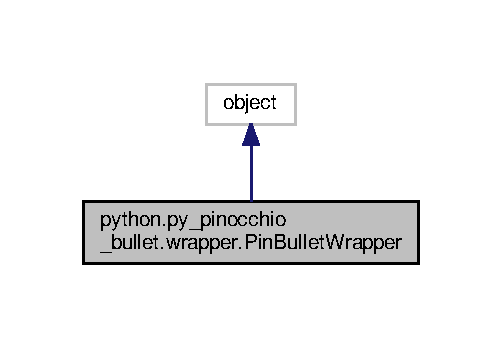
\includegraphics[width=241pt]{classpython_1_1py__pinocchio__bullet_1_1wrapper_1_1PinBulletWrapper__inherit__graph}
\end{center}
\end{figure}


Collaboration diagram for python.\+py\+\_\+pinocchio\+\_\+bullet.\+wrapper.\+Pin\+Bullet\+Wrapper\+:
\nopagebreak
\begin{figure}[H]
\begin{center}
\leavevmode
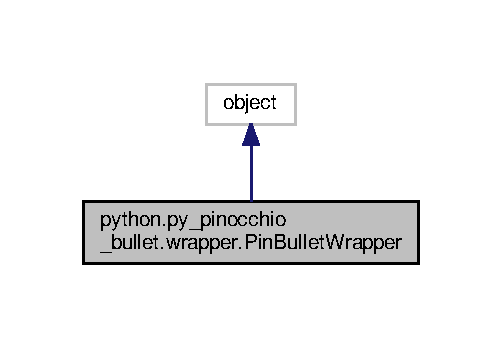
\includegraphics[width=241pt]{classpython_1_1py__pinocchio__bullet_1_1wrapper_1_1PinBulletWrapper__coll__graph}
\end{center}
\end{figure}
\subsection*{Public Member Functions}
\begin{DoxyCompactItemize}
\item 
def {\bfseries \+\_\+\+\_\+init\+\_\+\+\_\+} (self, robot\+\_\+id, pinocchio\+\_\+robot, joint\+\_\+names, endeff\+\_\+names, use\+Fixed\+Base=False)\hypertarget{classpython_1_1py__pinocchio__bullet_1_1wrapper_1_1PinBulletWrapper_ad50c0916de58d6c8eda6dcfa81e84b9d}{}\label{classpython_1_1py__pinocchio__bullet_1_1wrapper_1_1PinBulletWrapper_ad50c0916de58d6c8eda6dcfa81e84b9d}

\item 
def \hyperlink{classpython_1_1py__pinocchio__bullet_1_1wrapper_1_1PinBulletWrapper_ab91d7c32be024c5d90bbb7af527313fb}{get\+\_\+force} (self)\hypertarget{classpython_1_1py__pinocchio__bullet_1_1wrapper_1_1PinBulletWrapper_ab91d7c32be024c5d90bbb7af527313fb}{}\label{classpython_1_1py__pinocchio__bullet_1_1wrapper_1_1PinBulletWrapper_ab91d7c32be024c5d90bbb7af527313fb}

\begin{DoxyCompactList}\small\item\em Returns the force readings as well as the set of active contacts. \end{DoxyCompactList}\item 
def \hyperlink{classpython_1_1py__pinocchio__bullet_1_1wrapper_1_1PinBulletWrapper_af3f64a253e479c47111b4cba94dfd77a}{get\+\_\+base\+\_\+velocity\+\_\+world} (self)
\begin{DoxyCompactList}\small\item\em Returns the velocity of the base in the world frame. \end{DoxyCompactList}\item 
def {\bfseries get\+\_\+state} (self)\hypertarget{classpython_1_1py__pinocchio__bullet_1_1wrapper_1_1PinBulletWrapper_a35ba3a21b8b36df34d1ad8389f4c4caa}{}\label{classpython_1_1py__pinocchio__bullet_1_1wrapper_1_1PinBulletWrapper_a35ba3a21b8b36df34d1ad8389f4c4caa}

\item 
def \hyperlink{classpython_1_1py__pinocchio__bullet_1_1wrapper_1_1PinBulletWrapper_a2c79661f50580185498007e5755c774d}{update\+\_\+pinocchio} (self, q, dq)
\begin{DoxyCompactList}\small\item\em Updates the pinocchio robot. \end{DoxyCompactList}\item 
def \hyperlink{classpython_1_1py__pinocchio__bullet_1_1wrapper_1_1PinBulletWrapper_ab4ea626824c8043f48aa3c57b7504426}{get\+\_\+state\+\_\+update\+\_\+pinocchio} (self)
\begin{DoxyCompactList}\small\item\em Get state from pybullet and update pinocchio robot internals. \end{DoxyCompactList}\item 
def {\bfseries reset\+\_\+state} (self, q, dq)\hypertarget{classpython_1_1py__pinocchio__bullet_1_1wrapper_1_1PinBulletWrapper_a99f63187e0e22633340040f4451fe137}{}\label{classpython_1_1py__pinocchio__bullet_1_1wrapper_1_1PinBulletWrapper_a99f63187e0e22633340040f4451fe137}

\item 
def {\bfseries send\+\_\+joint\+\_\+command} (self, tau)\hypertarget{classpython_1_1py__pinocchio__bullet_1_1wrapper_1_1PinBulletWrapper_a6c97fd610f27ceeb781124933ca94c45}{}\label{classpython_1_1py__pinocchio__bullet_1_1wrapper_1_1PinBulletWrapper_a6c97fd610f27ceeb781124933ca94c45}

\end{DoxyCompactItemize}
\subsection*{Public Attributes}
\begin{DoxyCompactItemize}
\item 
{\bfseries nq}\hypertarget{classpython_1_1py__pinocchio__bullet_1_1wrapper_1_1PinBulletWrapper_a991baba630bdd4a7d6d5be186d695b15}{}\label{classpython_1_1py__pinocchio__bullet_1_1wrapper_1_1PinBulletWrapper_a991baba630bdd4a7d6d5be186d695b15}

\item 
{\bfseries nv}\hypertarget{classpython_1_1py__pinocchio__bullet_1_1wrapper_1_1PinBulletWrapper_a935e2794645c3142ada1e291ba71669a}{}\label{classpython_1_1py__pinocchio__bullet_1_1wrapper_1_1PinBulletWrapper_a935e2794645c3142ada1e291ba71669a}

\item 
{\bfseries nj}\hypertarget{classpython_1_1py__pinocchio__bullet_1_1wrapper_1_1PinBulletWrapper_acad3358e0076a280c0b4a3ee6f04e8f2}{}\label{classpython_1_1py__pinocchio__bullet_1_1wrapper_1_1PinBulletWrapper_acad3358e0076a280c0b4a3ee6f04e8f2}

\item 
{\bfseries nf}\hypertarget{classpython_1_1py__pinocchio__bullet_1_1wrapper_1_1PinBulletWrapper_aa1df78496c40d13f5c21ffb647cd1c44}{}\label{classpython_1_1py__pinocchio__bullet_1_1wrapper_1_1PinBulletWrapper_aa1df78496c40d13f5c21ffb647cd1c44}

\item 
{\bfseries robot\+\_\+id}\hypertarget{classpython_1_1py__pinocchio__bullet_1_1wrapper_1_1PinBulletWrapper_a88cff7be8db6447db6a003e93a8be3e2}{}\label{classpython_1_1py__pinocchio__bullet_1_1wrapper_1_1PinBulletWrapper_a88cff7be8db6447db6a003e93a8be3e2}

\item 
{\bfseries pinocchio\+\_\+robot}\hypertarget{classpython_1_1py__pinocchio__bullet_1_1wrapper_1_1PinBulletWrapper_a2a125c40aecef05dc101bcf5df1acd4a}{}\label{classpython_1_1py__pinocchio__bullet_1_1wrapper_1_1PinBulletWrapper_a2a125c40aecef05dc101bcf5df1acd4a}

\item 
{\bfseries use\+Fixed\+Base}\hypertarget{classpython_1_1py__pinocchio__bullet_1_1wrapper_1_1PinBulletWrapper_a7d3dd146b61385b8918ca169caa186de}{}\label{classpython_1_1py__pinocchio__bullet_1_1wrapper_1_1PinBulletWrapper_a7d3dd146b61385b8918ca169caa186de}

\item 
{\bfseries joint\+\_\+names}\hypertarget{classpython_1_1py__pinocchio__bullet_1_1wrapper_1_1PinBulletWrapper_a7c8f9529af82c7800dd09937f2845488}{}\label{classpython_1_1py__pinocchio__bullet_1_1wrapper_1_1PinBulletWrapper_a7c8f9529af82c7800dd09937f2845488}

\item 
{\bfseries endeff\+\_\+names}\hypertarget{classpython_1_1py__pinocchio__bullet_1_1wrapper_1_1PinBulletWrapper_ad5840b635e53996b2f811ff377765420}{}\label{classpython_1_1py__pinocchio__bullet_1_1wrapper_1_1PinBulletWrapper_ad5840b635e53996b2f811ff377765420}

\item 
{\bfseries bullet\+\_\+joint\+\_\+ids}\hypertarget{classpython_1_1py__pinocchio__bullet_1_1wrapper_1_1PinBulletWrapper_a1a6ce8db04a37ee71171676092771df9}{}\label{classpython_1_1py__pinocchio__bullet_1_1wrapper_1_1PinBulletWrapper_a1a6ce8db04a37ee71171676092771df9}

\item 
{\bfseries pinocchio\+\_\+joint\+\_\+ids}\hypertarget{classpython_1_1py__pinocchio__bullet_1_1wrapper_1_1PinBulletWrapper_a8213dc2be44eb764b4abb5a28b7d59b4}{}\label{classpython_1_1py__pinocchio__bullet_1_1wrapper_1_1PinBulletWrapper_a8213dc2be44eb764b4abb5a28b7d59b4}

\item 
{\bfseries pin2bullet\+\_\+joint\+\_\+only\+\_\+array}\hypertarget{classpython_1_1py__pinocchio__bullet_1_1wrapper_1_1PinBulletWrapper_a66629feee901449769b8ad08355c556f}{}\label{classpython_1_1py__pinocchio__bullet_1_1wrapper_1_1PinBulletWrapper_a66629feee901449769b8ad08355c556f}

\item 
{\bfseries bullet\+\_\+endeff\+\_\+ids}\hypertarget{classpython_1_1py__pinocchio__bullet_1_1wrapper_1_1PinBulletWrapper_a5e929f341225057ec66f9d88f5bf4649}{}\label{classpython_1_1py__pinocchio__bullet_1_1wrapper_1_1PinBulletWrapper_a5e929f341225057ec66f9d88f5bf4649}

\item 
{\bfseries pinocchio\+\_\+endeff\+\_\+ids}\hypertarget{classpython_1_1py__pinocchio__bullet_1_1wrapper_1_1PinBulletWrapper_afd4d3e0702d0e46f9898ff3334d225d2}{}\label{classpython_1_1py__pinocchio__bullet_1_1wrapper_1_1PinBulletWrapper_afd4d3e0702d0e46f9898ff3334d225d2}

\end{DoxyCompactItemize}
\subsection*{Private Member Functions}
\begin{DoxyCompactItemize}
\item 
def {\bfseries \+\_\+action} (self, pos, rot)\hypertarget{classpython_1_1py__pinocchio__bullet_1_1wrapper_1_1PinBulletWrapper_ab40bb4a94859d3bad4d22f00ab47450d}{}\label{classpython_1_1py__pinocchio__bullet_1_1wrapper_1_1PinBulletWrapper_ab40bb4a94859d3bad4d22f00ab47450d}

\end{DoxyCompactItemize}


\subsection{Member Function Documentation}
\index{python\+::py\+\_\+pinocchio\+\_\+bullet\+::wrapper\+::\+Pin\+Bullet\+Wrapper@{python\+::py\+\_\+pinocchio\+\_\+bullet\+::wrapper\+::\+Pin\+Bullet\+Wrapper}!get\+\_\+base\+\_\+velocity\+\_\+world@{get\+\_\+base\+\_\+velocity\+\_\+world}}
\index{get\+\_\+base\+\_\+velocity\+\_\+world@{get\+\_\+base\+\_\+velocity\+\_\+world}!python\+::py\+\_\+pinocchio\+\_\+bullet\+::wrapper\+::\+Pin\+Bullet\+Wrapper@{python\+::py\+\_\+pinocchio\+\_\+bullet\+::wrapper\+::\+Pin\+Bullet\+Wrapper}}
\subsubsection[{\texorpdfstring{get\+\_\+base\+\_\+velocity\+\_\+world(self)}{get_base_velocity_world(self)}}]{\setlength{\rightskip}{0pt plus 5cm}def python.\+py\+\_\+pinocchio\+\_\+bullet.\+wrapper.\+Pin\+Bullet\+Wrapper.\+get\+\_\+base\+\_\+velocity\+\_\+world (
\begin{DoxyParamCaption}
\item[{}]{self}
\end{DoxyParamCaption}
)}\hypertarget{classpython_1_1py__pinocchio__bullet_1_1wrapper_1_1PinBulletWrapper_af3f64a253e479c47111b4cba94dfd77a}{}\label{classpython_1_1py__pinocchio__bullet_1_1wrapper_1_1PinBulletWrapper_af3f64a253e479c47111b4cba94dfd77a}


Returns the velocity of the base in the world frame. 

\begin{DoxyReturn}{Returns}
np.\+array((6,1)) with the translation and angular velocity 
\end{DoxyReturn}
\index{python\+::py\+\_\+pinocchio\+\_\+bullet\+::wrapper\+::\+Pin\+Bullet\+Wrapper@{python\+::py\+\_\+pinocchio\+\_\+bullet\+::wrapper\+::\+Pin\+Bullet\+Wrapper}!get\+\_\+state\+\_\+update\+\_\+pinocchio@{get\+\_\+state\+\_\+update\+\_\+pinocchio}}
\index{get\+\_\+state\+\_\+update\+\_\+pinocchio@{get\+\_\+state\+\_\+update\+\_\+pinocchio}!python\+::py\+\_\+pinocchio\+\_\+bullet\+::wrapper\+::\+Pin\+Bullet\+Wrapper@{python\+::py\+\_\+pinocchio\+\_\+bullet\+::wrapper\+::\+Pin\+Bullet\+Wrapper}}
\subsubsection[{\texorpdfstring{get\+\_\+state\+\_\+update\+\_\+pinocchio(self)}{get_state_update_pinocchio(self)}}]{\setlength{\rightskip}{0pt plus 5cm}def python.\+py\+\_\+pinocchio\+\_\+bullet.\+wrapper.\+Pin\+Bullet\+Wrapper.\+get\+\_\+state\+\_\+update\+\_\+pinocchio (
\begin{DoxyParamCaption}
\item[{}]{self}
\end{DoxyParamCaption}
)}\hypertarget{classpython_1_1py__pinocchio__bullet_1_1wrapper_1_1PinBulletWrapper_ab4ea626824c8043f48aa3c57b7504426}{}\label{classpython_1_1py__pinocchio__bullet_1_1wrapper_1_1PinBulletWrapper_ab4ea626824c8043f48aa3c57b7504426}


Get state from pybullet and update pinocchio robot internals. 

This gets the state from the pybullet simulator and forwards the kinematics, jacobians, centroidal moments on the pinocchio robot (see forward\+\_\+pinocchio for details on computed quantities). \index{python\+::py\+\_\+pinocchio\+\_\+bullet\+::wrapper\+::\+Pin\+Bullet\+Wrapper@{python\+::py\+\_\+pinocchio\+\_\+bullet\+::wrapper\+::\+Pin\+Bullet\+Wrapper}!update\+\_\+pinocchio@{update\+\_\+pinocchio}}
\index{update\+\_\+pinocchio@{update\+\_\+pinocchio}!python\+::py\+\_\+pinocchio\+\_\+bullet\+::wrapper\+::\+Pin\+Bullet\+Wrapper@{python\+::py\+\_\+pinocchio\+\_\+bullet\+::wrapper\+::\+Pin\+Bullet\+Wrapper}}
\subsubsection[{\texorpdfstring{update\+\_\+pinocchio(self, q, dq)}{update_pinocchio(self, q, dq)}}]{\setlength{\rightskip}{0pt plus 5cm}def python.\+py\+\_\+pinocchio\+\_\+bullet.\+wrapper.\+Pin\+Bullet\+Wrapper.\+update\+\_\+pinocchio (
\begin{DoxyParamCaption}
\item[{}]{self, }
\item[{}]{q, }
\item[{}]{dq}
\end{DoxyParamCaption}
)}\hypertarget{classpython_1_1py__pinocchio__bullet_1_1wrapper_1_1PinBulletWrapper_a2c79661f50580185498007e5755c774d}{}\label{classpython_1_1py__pinocchio__bullet_1_1wrapper_1_1PinBulletWrapper_a2c79661f50580185498007e5755c774d}


Updates the pinocchio robot. 

This includes updating\+:
\begin{DoxyItemize}
\item kinematics
\item joint and frame jacobian
\item centroidal momentum
\end{DoxyItemize}


\begin{DoxyParams}{Parameters}
{\em q} & Pinocchio generalized position vect. \\
\hline
{\em dq} & Pinocchio generalize velocity vector. \\
\hline
\end{DoxyParams}


The documentation for this class was generated from the following file\+:\begin{DoxyCompactItemize}
\item 
python/py\+\_\+pinocchio\+\_\+bullet/wrapper.\+py\end{DoxyCompactItemize}

\hypertarget{classquadruped_1_1QuadrupedRobot}{}\section{quadruped.\+Quadruped\+Robot Class Reference}
\label{classquadruped_1_1QuadrupedRobot}\index{quadruped.\+Quadruped\+Robot@{quadruped.\+Quadruped\+Robot}}


Inheritance diagram for quadruped.\+Quadruped\+Robot\+:
\nopagebreak
\begin{figure}[H]
\begin{center}
\leavevmode
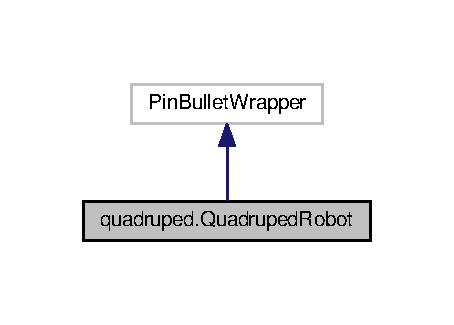
\includegraphics[width=218pt]{classquadruped_1_1QuadrupedRobot__inherit__graph}
\end{center}
\end{figure}


Collaboration diagram for quadruped.\+Quadruped\+Robot\+:
\nopagebreak
\begin{figure}[H]
\begin{center}
\leavevmode
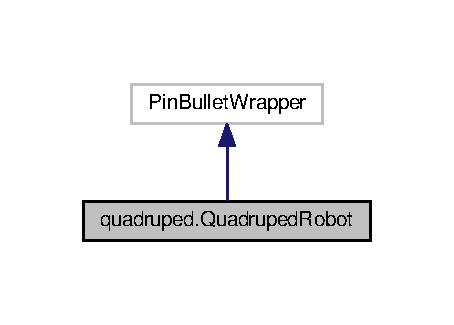
\includegraphics[width=218pt]{classquadruped_1_1QuadrupedRobot__coll__graph}
\end{center}
\end{figure}
\subsection*{Public Member Functions}
\begin{DoxyCompactItemize}
\item 
def {\bfseries \+\_\+\+\_\+init\+\_\+\+\_\+} (self, physics\+Client=None)\hypertarget{classquadruped_1_1QuadrupedRobot_acd22d681511fc02910f6dd168f3e6305}{}\label{classquadruped_1_1QuadrupedRobot_acd22d681511fc02910f6dd168f3e6305}

\end{DoxyCompactItemize}
\subsection*{Public Attributes}
\begin{DoxyCompactItemize}
\item 
{\bfseries physics\+Client}\hypertarget{classquadruped_1_1QuadrupedRobot_aa887aeaac1b638e055e79f18e03a045d}{}\label{classquadruped_1_1QuadrupedRobot_aa887aeaac1b638e055e79f18e03a045d}

\item 
{\bfseries plane\+Id}\hypertarget{classquadruped_1_1QuadrupedRobot_a49f5fd9cb0672ae09162c99646ac5445}{}\label{classquadruped_1_1QuadrupedRobot_a49f5fd9cb0672ae09162c99646ac5445}

\item 
{\bfseries urdf\+\_\+path}\hypertarget{classquadruped_1_1QuadrupedRobot_a467b697aeca43fd6864e6cd022046aa6}{}\label{classquadruped_1_1QuadrupedRobot_a467b697aeca43fd6864e6cd022046aa6}

\item 
{\bfseries robot\+Id}\hypertarget{classquadruped_1_1QuadrupedRobot_a105f6c0b8ffc1d09f9131934608a20dd}{}\label{classquadruped_1_1QuadrupedRobot_a105f6c0b8ffc1d09f9131934608a20dd}

\item 
{\bfseries pin\+\_\+robot}\hypertarget{classquadruped_1_1QuadrupedRobot_a5a3e8b0ed6f8b333adb8c9416b394d11}{}\label{classquadruped_1_1QuadrupedRobot_a5a3e8b0ed6f8b333adb8c9416b394d11}

\item 
{\bfseries base\+\_\+link\+\_\+name}\hypertarget{classquadruped_1_1QuadrupedRobot_ad5320c45135714963a6f8cd85f8eaef7}{}\label{classquadruped_1_1QuadrupedRobot_ad5320c45135714963a6f8cd85f8eaef7}

\item 
{\bfseries joint\+\_\+names}\hypertarget{classquadruped_1_1QuadrupedRobot_ac5b376bb29520b25119944ee667987f2}{}\label{classquadruped_1_1QuadrupedRobot_ac5b376bb29520b25119944ee667987f2}

\end{DoxyCompactItemize}


The documentation for this class was generated from the following file\+:\begin{DoxyCompactItemize}
\item 
demo/quadruped.\+py\end{DoxyCompactItemize}

%--- End generated contents ---

% Index
\backmatter
\newpage
\phantomsection
\clearemptydoublepage
\addcontentsline{toc}{chapter}{Index}
\printindex

\end{document}
